% Created by tikzDevice version 0.10.1 on 2017-11-24 11:28:21
% !TEX encoding = UTF-8 Unicode
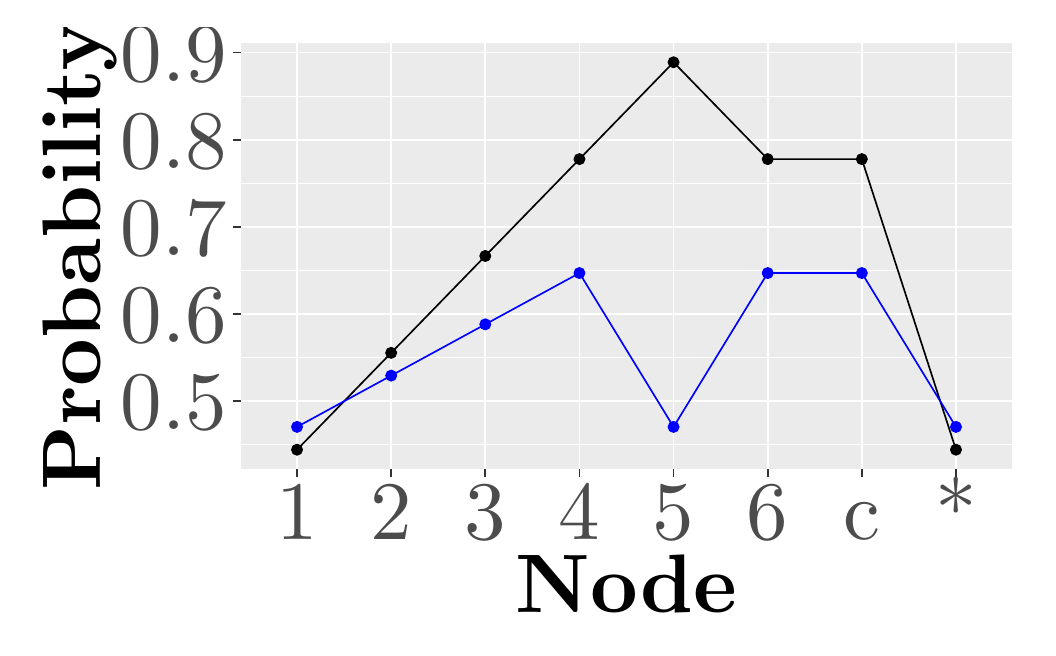
\begin{tikzpicture}[x=1pt,y=1pt]
\definecolor{fillColor}{RGB}{255,255,255}
\path[use as bounding box,fill=fillColor,fill opacity=0.00] (0,0) rectangle (361.35,216.81);
\begin{scope}
\path[clip] (  0.00,  0.00) rectangle (361.35,216.81);
\definecolor{drawColor}{RGB}{255,255,255}
\definecolor{fillColor}{RGB}{255,255,255}

\path[draw=drawColor,line width= 0.6pt,line join=round,line cap=round,fill=fillColor] (  0.00,  0.00) rectangle (361.35,216.81);
\end{scope}
\begin{scope}
\path[clip] ( 76.92, 57.31) rectangle (355.85,211.31);
\definecolor{fillColor}{gray}{0.92}

\path[fill=fillColor] ( 76.92, 57.31) rectangle (355.85,211.31);
\definecolor{drawColor}{RGB}{255,255,255}

\path[draw=drawColor,line width= 0.3pt,line join=round] ( 76.92, 66.06) --
	(355.85, 66.06);

\path[draw=drawColor,line width= 0.3pt,line join=round] ( 76.92, 97.56) --
	(355.85, 97.56);

\path[draw=drawColor,line width= 0.3pt,line join=round] ( 76.92,129.06) --
	(355.85,129.06);

\path[draw=drawColor,line width= 0.3pt,line join=round] ( 76.92,160.56) --
	(355.85,160.56);

\path[draw=drawColor,line width= 0.3pt,line join=round] ( 76.92,192.06) --
	(355.85,192.06);

\path[draw=drawColor,line width= 0.6pt,line join=round] ( 76.92, 81.81) --
	(355.85, 81.81);

\path[draw=drawColor,line width= 0.6pt,line join=round] ( 76.92,113.31) --
	(355.85,113.31);

\path[draw=drawColor,line width= 0.6pt,line join=round] ( 76.92,144.81) --
	(355.85,144.81);

\path[draw=drawColor,line width= 0.6pt,line join=round] ( 76.92,176.31) --
	(355.85,176.31);

\path[draw=drawColor,line width= 0.6pt,line join=round] ( 76.92,207.81) --
	(355.85,207.81);

\path[draw=drawColor,line width= 0.6pt,line join=round] ( 97.33, 57.31) --
	( 97.33,211.31);

\path[draw=drawColor,line width= 0.6pt,line join=round] (131.35, 57.31) --
	(131.35,211.31);

\path[draw=drawColor,line width= 0.6pt,line join=round] (165.36, 57.31) --
	(165.36,211.31);

\path[draw=drawColor,line width= 0.6pt,line join=round] (199.38, 57.31) --
	(199.38,211.31);

\path[draw=drawColor,line width= 0.6pt,line join=round] (233.39, 57.31) --
	(233.39,211.31);

\path[draw=drawColor,line width= 0.6pt,line join=round] (267.41, 57.31) --
	(267.41,211.31);

\path[draw=drawColor,line width= 0.6pt,line join=round] (301.42, 57.31) --
	(301.42,211.31);

\path[draw=drawColor,line width= 0.6pt,line join=round] (335.44, 57.31) --
	(335.44,211.31);
\definecolor{drawColor}{RGB}{0,0,0}
\definecolor{fillColor}{RGB}{0,0,0}

\path[draw=drawColor,line width= 0.4pt,line join=round,line cap=round,fill=fillColor] ( 97.33, 64.31) circle (  1.96);

\path[draw=drawColor,line width= 0.4pt,line join=round,line cap=round,fill=fillColor] (131.35, 99.31) circle (  1.96);

\path[draw=drawColor,line width= 0.4pt,line join=round,line cap=round,fill=fillColor] (165.36,134.31) circle (  1.96);

\path[draw=drawColor,line width= 0.4pt,line join=round,line cap=round,fill=fillColor] (199.38,169.31) circle (  1.96);

\path[draw=drawColor,line width= 0.4pt,line join=round,line cap=round,fill=fillColor] (233.39,204.31) circle (  1.96);

\path[draw=drawColor,line width= 0.4pt,line join=round,line cap=round,fill=fillColor] (267.41,169.31) circle (  1.96);

\path[draw=drawColor,line width= 0.4pt,line join=round,line cap=round,fill=fillColor] (301.42,169.31) circle (  1.96);

\path[draw=drawColor,line width= 0.4pt,line join=round,line cap=round,fill=fillColor] (335.44, 64.31) circle (  1.96);

\path[draw=drawColor,line width= 0.6pt,line join=round] ( 97.33, 64.31) --
	(131.35, 99.31) --
	(165.36,134.31) --
	(199.38,169.31) --
	(233.39,204.31) --
	(267.41,169.31) --
	(301.42,169.31) --
	(335.44, 64.31);
\definecolor{drawColor}{RGB}{0,0,255}
\definecolor{fillColor}{RGB}{0,0,255}

\path[draw=drawColor,line width= 0.4pt,line join=round,line cap=round,fill=fillColor] ( 97.33, 72.55) circle (  1.96);

\path[draw=drawColor,line width= 0.4pt,line join=round,line cap=round,fill=fillColor] (131.35, 91.08) circle (  1.96);

\path[draw=drawColor,line width= 0.4pt,line join=round,line cap=round,fill=fillColor] (165.36,109.61) circle (  1.96);

\path[draw=drawColor,line width= 0.4pt,line join=round,line cap=round,fill=fillColor] (199.38,128.14) circle (  1.96);

\path[draw=drawColor,line width= 0.4pt,line join=round,line cap=round,fill=fillColor] (233.39, 72.55) circle (  1.96);

\path[draw=drawColor,line width= 0.4pt,line join=round,line cap=round,fill=fillColor] (267.41,128.14) circle (  1.96);

\path[draw=drawColor,line width= 0.4pt,line join=round,line cap=round,fill=fillColor] (301.42,128.14) circle (  1.96);

\path[draw=drawColor,line width= 0.4pt,line join=round,line cap=round,fill=fillColor] (335.44, 72.55) circle (  1.96);

\path[draw=drawColor,line width= 0.6pt,line join=round] ( 97.33, 72.55) --
	(131.35, 91.08) --
	(165.36,109.61) --
	(199.38,128.14) --
	(233.39, 72.55) --
	(267.41,128.14) --
	(301.42,128.14) --
	(335.44, 72.55);
\end{scope}
\begin{scope}
\path[clip] (  0.00,  0.00) rectangle (361.35,216.81);
\definecolor{drawColor}{gray}{0.30}

\node[text=drawColor,anchor=base east,inner sep=0pt, outer sep=0pt, scale=  3.00] at ( 71.97, 71.48) {0.5};

\node[text=drawColor,anchor=base east,inner sep=0pt, outer sep=0pt, scale=  3.00] at ( 71.97,102.98) {0.6};

\node[text=drawColor,anchor=base east,inner sep=0pt, outer sep=0pt, scale=  3.00] at ( 71.97,134.48) {0.7};

\node[text=drawColor,anchor=base east,inner sep=0pt, outer sep=0pt, scale=  3.00] at ( 71.97,165.98) {0.8};

\node[text=drawColor,anchor=base east,inner sep=0pt, outer sep=0pt, scale=  3.00] at ( 71.97,197.48) {0.9};
\end{scope}
\begin{scope}
\path[clip] (  0.00,  0.00) rectangle (361.35,216.81);
\definecolor{drawColor}{gray}{0.20}

\path[draw=drawColor,line width= 0.6pt,line join=round] ( 74.17, 81.81) --
	( 76.92, 81.81);

\path[draw=drawColor,line width= 0.6pt,line join=round] ( 74.17,113.31) --
	( 76.92,113.31);

\path[draw=drawColor,line width= 0.6pt,line join=round] ( 74.17,144.81) --
	( 76.92,144.81);

\path[draw=drawColor,line width= 0.6pt,line join=round] ( 74.17,176.31) --
	( 76.92,176.31);

\path[draw=drawColor,line width= 0.6pt,line join=round] ( 74.17,207.81) --
	( 76.92,207.81);
\end{scope}
\begin{scope}
\path[clip] (  0.00,  0.00) rectangle (361.35,216.81);
\definecolor{drawColor}{gray}{0.20}

\path[draw=drawColor,line width= 0.6pt,line join=round] ( 97.33, 54.56) --
	( 97.33, 57.31);

\path[draw=drawColor,line width= 0.6pt,line join=round] (131.35, 54.56) --
	(131.35, 57.31);

\path[draw=drawColor,line width= 0.6pt,line join=round] (165.36, 54.56) --
	(165.36, 57.31);

\path[draw=drawColor,line width= 0.6pt,line join=round] (199.38, 54.56) --
	(199.38, 57.31);

\path[draw=drawColor,line width= 0.6pt,line join=round] (233.39, 54.56) --
	(233.39, 57.31);

\path[draw=drawColor,line width= 0.6pt,line join=round] (267.41, 54.56) --
	(267.41, 57.31);

\path[draw=drawColor,line width= 0.6pt,line join=round] (301.42, 54.56) --
	(301.42, 57.31);

\path[draw=drawColor,line width= 0.6pt,line join=round] (335.44, 54.56) --
	(335.44, 57.31);
\end{scope}
\begin{scope}
\path[clip] (  0.00,  0.00) rectangle (361.35,216.81);
\definecolor{drawColor}{gray}{0.30}

\node[text=drawColor,anchor=base,inner sep=0pt, outer sep=0pt, scale=  3.00] at ( 97.33, 31.70) {1};

\node[text=drawColor,anchor=base,inner sep=0pt, outer sep=0pt, scale=  3.00] at (131.35, 31.70) {2};

\node[text=drawColor,anchor=base,inner sep=0pt, outer sep=0pt, scale=  3.00] at (165.36, 31.70) {3};

\node[text=drawColor,anchor=base,inner sep=0pt, outer sep=0pt, scale=  3.00] at (199.38, 31.70) {4};

\node[text=drawColor,anchor=base,inner sep=0pt, outer sep=0pt, scale=  3.00] at (233.39, 31.70) {5};

\node[text=drawColor,anchor=base,inner sep=0pt, outer sep=0pt, scale=  3.00] at (267.41, 31.70) {6};

\node[text=drawColor,anchor=base,inner sep=0pt, outer sep=0pt, scale=  3.00] at (301.42, 31.70) {c};

\node[text=drawColor,anchor=base,inner sep=0pt, outer sep=0pt, scale=  3.00] at (335.44, 31.70) {*};
\end{scope}
\begin{scope}
\path[clip] (  0.00,  0.00) rectangle (361.35,216.81);
\definecolor{drawColor}{RGB}{0,0,0}

\node[text=drawColor,anchor=base,inner sep=0pt, outer sep=0pt, scale=  3.00] at (216.39,  5.50) {\bfseries Node};
\end{scope}
\begin{scope}
\path[clip] (  0.00,  0.00) rectangle (361.35,216.81);
\definecolor{drawColor}{RGB}{0,0,0}

\node[text=drawColor,rotate= 90.00,anchor=base,inner sep=0pt, outer sep=0pt, scale=  3.00] at ( 26.20,134.31) {\bfseries Probability};
\end{scope}
\end{tikzpicture}
